\documentclass[tikz, border=5mm]{standalone}
\usepackage{tikz}
\usetikzlibrary{shapes.geometric, arrows, positioning, fit, calc}
\usepackage{fontspec}
\setmainfont{Times New Roman}
\begin{document}
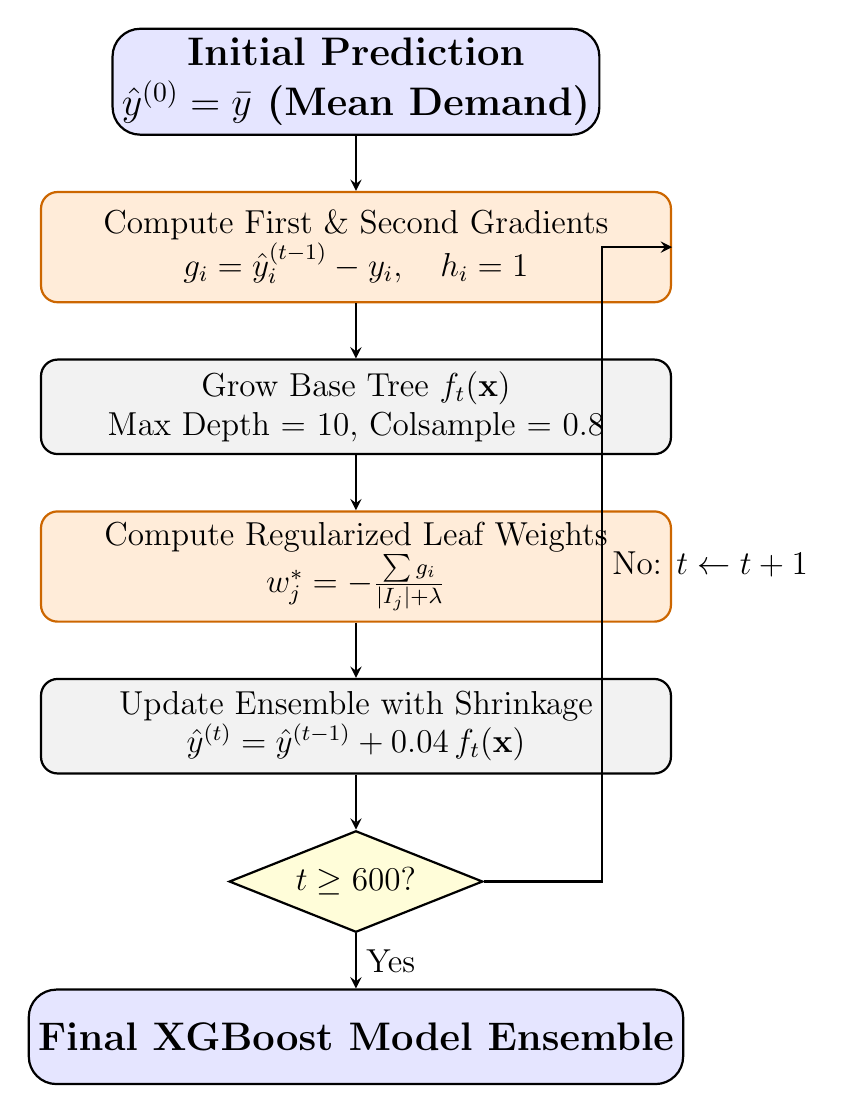
\begin{tikzpicture}[
    node distance=0.7cm,
    startstop/.style={rectangle, rounded corners=10pt, minimum width=6cm, minimum height=1.2cm, align=center, draw=black, thick, fill=blue!10, font=\rmfamily\bfseries\Large},
    block/.style={rectangle, rounded corners=6pt, minimum width=8cm, minimum height=1.2cm, align=center, draw=black, thick, fill=gray!10, font=\rmfamily\large},
    math/.style={rectangle, rounded corners=6pt, minimum width=8cm, minimum height=1.4cm, align=center, draw=orange!80!black, thick, fill=orange!15, font=\rmfamily\large},
    decision/.style={diamond, aspect=2.5, minimum width=3cm, draw=black, thick, fill=yellow!15, font=\rmfamily\large, align=center},
    arrow/.style={thick,->,>=stealth}
]
\node (init) [startstop] {Initial Prediction\\$\hat{y}^{(0)} = \bar{y}$ (Mean Demand)};
\node (grad) [math, below=of init] {Compute First \& Second Gradients\\$g_i = \hat{y}_i^{(t-1)} - y_i, \quad h_i = 1$};
\node (tree) [block, below=of grad] {Grow Base Tree $f_t(\mathbf{x})$\\Max Depth = 10, Colsample = 0.8};
\node (leaf) [math, below=of tree] {Compute Regularized Leaf Weights\\$w_j^* = -\frac{\sum g_i}{|I_j| + \lambda}$};
\node (update) [block, below=of leaf] {Update Ensemble with Shrinkage\\$\hat{y}^{(t)} = \hat{y}^{(t-1)} + 0.04 \, f_t(\mathbf{x})$};
\node (check) [decision, below=of update] {$t \ge 600$?};
\node (final) [startstop, below=of check] {Final XGBoost Model Ensemble};

\draw [arrow] (init) -- (grad);
\draw [arrow] (grad) -- (tree);
\draw [arrow] (tree) -- (leaf);
\draw [arrow] (leaf) -- (update);
\draw [arrow] (update) -- (check);
\draw [arrow] (check) -- node[right, font=\large] {Yes} (final);
\draw [arrow] (check.east) -- ++(1.5,0) |- node[near start, right, font=\large] {No: $t \leftarrow t + 1$} (grad.east);
\end{tikzpicture}
\end{document}
